\begin{thm}{230}{\hosi 6}{京レ (2019)}
 $t$を正の実数とし、直線$\mr{L}:$~$y=t$ と、曲線$\mr{K}:$~$y=\left|\log (1+x)\right|$~$(x>-1)$ の2交点を$\mr{A, B}$とする。$\mr{A, B}$における$\mr{K}$の接線の交点を$\mr{C}$とし、$\triangle\mr{ABC}$の外接円$\mr{E}$の面積を$S(t)$とする。$\disp \lim_{t\to +0} \frac{S(t)}{t^2}$ を求めよ。
\end{thm}

2交点のうち、$x$座標が負のものを$\mr{A}$、正のものを$\mr{B}$とする。
\begin{figure}[H]
 \centering
 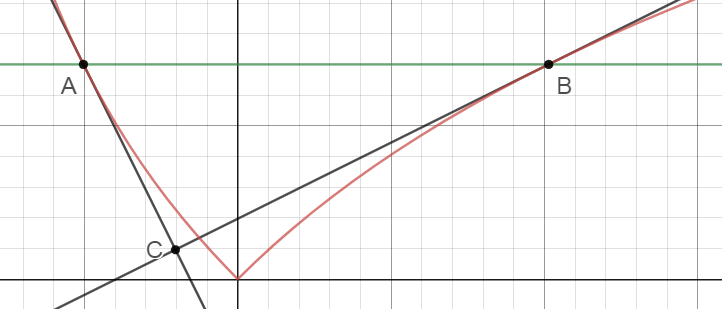
\includegraphics[width=0.8\linewidth]{../problems/Q_230/A_230.png}
\end{figure}

曲線$\mr{K}$は、$-1<x\le 0$で$y=-\log(1+x)$なので、$\mr{A}$の$x$座標は
\[ -\log(1+x)=t \quad\dou\quad x=e^{-t}-1 \]
$y'=-\dfrac{1}{1+x}$より、点$\mr{A}$での接線は、
\[ y=-e^tx+1+t-e^t \]
一方、曲線$\mr{K}$は$x\ge 0$で$y=\log(1+x)$なので、$\mr{B}$の$x$座標は
\[ \log(1+x)=t \quad\dou\quad x=e^t-1 \]
$y'=\dfrac{1}{1+x}$より、点$\mr{B}$での接線は、
\[ y=e^{-t}x-1+t+e^{-t} \]
これら2本の接線は直交するから、$\triangle\mr{ABC}$は$\angle\mr{C}$が直角な直角三角形となる。したがって、$\triangle\mr{ABC}$の外心は$\mr{AB}$の中点にある。よって外接円の半径$R$は
\[ R=\frac{(e^t-1)-(e^{-t}-1)}{2}=\frac{e^t-e^{-t}}{2} \]
と求まる。$S(t)=\pi R^2$であることから、$\disp \lim_{t\to +0}\frac{R}{t}$を考えると、
\[  \lim_{t\to +0} \frac{R}{t} = \lim_{t\to +0} \frac{e^t-e^{-t}}{2t} \]
この極限を求めるために、次の関数を考える。
\[ f(x)=e^x-e^{-x}-2x \,,\,\, g(x)=2xe^x-(e^x-e^{-x}) \]
これらについて、微分すると
\[ f'(x)=2e^x-2 \,,\,\, g'(x)=2xe^x \]
であるから、任意の$x\ge 0$において$f'(x)\ge 0$, $g'(x)\ge 0$が成り立ち、$f(x)$, $g(x)$は単調増加である。さらに$f(0)=g(0)=0$より、任意の$x\ge 0$において$f(x)\ge 0$, $g(x)\ge 0$が成り立つ。したがって、
\[ 2x \le e^x-e^{-x}\le 2xe^x \quad\dou\quad 1\le \frac{e^x-e^{-x}}{2x}\le e^x \]
これについて$x\to +0$の極限を考えれば、$\disp \lim_{t\to +0} \frac{R}{t}=1$ が示される。

よって求める極限は、
\[ \lim_{t\to +0} \frac{S(t)}{t^2}=\lim_{t\to +0} \pi\left(\frac{e^t-e^{-t}}{2t}\right)^2 = \pi \]
